\documentclass[aps,prl,onecolumn,10pt,notitlepage,superscriptaddress,nofootinbib]{revtex4-2}
\usepackage{amsmath,amssymb,bm,graphicx,booktabs,longtable,array}
\usepackage{xcolor}
\graphicspath{{figures/}}

\newcommand{\CP}{\mathbb{CP}}
\newcommand{\ii}{\mathrm{i}}
\newcommand{\resultneeded}[1]{\textbf{\color{red!70!black}[RESULT NEEDED: #1]}}
\renewcommand{\theequation}{S\arabic{equation}}
\renewcommand{\thefigure}{S\arabic{figure}}
\renewcommand{\thetable}{S\arabic{table}}

\begin{document}
\title{Supplemental Material for ``Projective Outcome Geometry and Born-Like Dipoles in Unitary Many-Body Detectors''}
\author{Authors withheld for review}
\affiliation{Affiliation withheld for review}
\date{August 14, 2026}
\maketitle

This Supplemental Material fixes the mathematical conventions, proves the outcome-antipode and Haar results, reconciles the forward construction with the production calculation, and records the numerical methods and provenance.  It is single-column throughout.  The term ``collapse'' is operational: the construction identifies product boundary-compatible states, not a discontinuous global dynamics or a physical selection law.

\section{Forward pole construction}

Let $U:\mathbb C^2\otimes\mathbb C^d\rightarrow\mathbb C^2\otimes\mathbb C^d$ be unitary, with qubit index first and detector basis fixed,
\begin{equation}
 U=\begin{pmatrix}A&B\\C&D\end{pmatrix}.                                      \label{seq:block}
\end{equation}
Write the input qubit ray homogeneously as $q=[\alpha:\beta]\in\CP^1$ and let $\eta\neq0$ be a detector vector.  Direct block multiplication gives
\begin{equation}
U[(\alpha|0\rangle+\beta|1\rangle)\otimes\eta]
=|0\rangle\otimes(\alpha A+\beta B)\eta
+|1\rangle\otimes(\alpha C+\beta D)\eta.                                   \label{seq:action}
\end{equation}
Thus output pole $0$ requires
\begin{equation}
L_0(\alpha,\beta)\eta=(\alpha C+\beta D)\eta=0,                              \label{seq:l0}
\end{equation}
whereas pole $1$ requires $L_1(\alpha,\beta)\eta=(\alpha A+\beta B)\eta=0$.  Unitarity ensures that the surviving component in Eq.~\eqref{seq:action} is nonzero.  The affine coordinate $z=\beta/\alpha=e^{\ii\phi}\tan(\theta/2)$ gives $C+zD$ and $A+zB$; $[0:1]$, or $z=\infty$, remains part of the projective problem.

\section{Exact antipodal outcome duality}

Choose a representative with $|\alpha|^2+|\beta|^2=1$ and define its orthogonal coordinate
\begin{equation}
q^\perp=(-\bar\beta,\bar\alpha)^T,
\qquad
R_q=\begin{pmatrix}\alpha&-\bar\beta\\\beta&\bar\alpha\end{pmatrix}\in SU(2).
\end{equation}
The lower-left block of $V=U(R_q\otimes I_d)$ is $L_0(q)$ and the upper-right block is $L_1(q^\perp)$.  Jacobi's complementary-minor identity applied to the unitary $V$ yields
\begin{equation}
\det L_0(\alpha,\beta)
=(-1)^d\det U\,\overline{\det L_1(-\bar\beta,\bar\alpha)}.                   \label{seq:jacobi}
\end{equation}
Therefore $q$ is an outcome-$0$ root if and only if $q^\perp$ is an outcome-$1$ root.  Algebraic multiplicity is preserved.  In stereographic coordinates the map is
\begin{equation}
z\longmapsto z_\perp=-\frac{1}{\bar z},                                        \label{seq:antipode}
\end{equation}
with $0\leftrightarrow\infty$.  The two pencils are regular or singular together.

For identically processed empirical measures,
\begin{equation}
\rho_1(\Omega)=\rho_0(-\Omega),\qquad
a(-\Omega)=-a(\Omega).                                                         \label{seq:odd}
\end{equation}
Hence a spherical-harmonic expansion of the exact paired asymmetry contains only odd $\ell$.  A projective Born rule along $\hat{\bm n}$ is the $\ell=1$ field $a_{\rm B}=\hat{\bm n}\cdot\bm r$.  Equivalently, with $s_{\rm even}(\Omega)=\rho_0(\Omega)+\rho_0(-\Omega)$,
\begin{equation}
\rho_0(\Omega)=\frac{s_{\rm even}(\Omega)}{2}
\left[1+\hat{\bm n}\cdot\bm r(\Omega)\right].                              \label{seq:bornrho}
\end{equation}
The total density may be highly nonuniform.  For Born behavior, its normalized odd part must be a unit dipole.  Along $z$, Eq.~\eqref{seq:bornrho} is equivalent to $\rho_0(-\Omega)/\rho_0(\Omega)=\tan^2(\theta/2)$.

\section{Regular roots, infinity, and singular pencils}

For a regular pencil, $p_0(\alpha,\beta)=\det(\alpha C+\beta D)$ is a nonzero homogeneous polynomial of degree $d$.  It has exactly $d$ roots on $\CP^1$, counted with algebraic multiplicity.  This does not imply $d$ distinct Bloch points.  At a root $q_j$ with nullity $g_j$, compatible detector rays form $\CP^{g_j-1}$; algebraic multiplicity and nullity need not agree.

In the generalized-eigenvalue convention $bC\eta=aD\eta$, for which the forward coordinate is $z=-a/b$, a normalized residual should be evaluated without affine division:
\begin{equation}
r=\frac{\|bC\eta-aD\eta\|}
{(|b|\|C\|+|a|\|D\|)\|\eta\|}.                                               \label{seq:resid}
\end{equation}
A zero denominator coordinate is a root at infinity rather than a numerical failure.  QZ/generalized Schur methods avoid explicit inversion and preserve this structure~\cite{MolerStewart1973}.

If $p_0\equiv0$, the finite-root statement fails and the Kronecker structure is required.  Qubit--qubit SWAP is the clean example:
\begin{equation}
U_{\rm SWAP}(|q\rangle_Q|0\rangle_D)=|0\rangle_Q|q\rangle_D,
\end{equation}
so every input qubit reaches pole $0$.  Conversely, $U=I$ is regular but maximally degenerate: each outcome has one Bloch pole with algebraic multiplicity $d$ and a $d$-dimensional detector nullspace.

The full pole-preimage set $\mathcal L_k=U^\dagger(|k\rangle\otimes\mathcal H_D)$ is a $d$-dimensional linear subspace.  The special product cone is $\mathcal S_k=\mathcal L_k\cap\Sigma$, where $\Sigma$ is the Segre product cone.  If a regular pencil has two distinct qubit roots $q_1,q_2$, compatible detector vectors cannot be proportional: otherwise both detector blocks would share a kernel and the pencil would be singular.  The sum $q_1\otimes\eta_1+q_2\otimes\eta_2$ therefore has Schmidt rank two.  Generic nonadditivity belongs to the product intersection $\mathcal S_k$, not to the linear preimage space $\mathcal L_k$.

\section{Haar roots are exactly the spherical ensemble}

For the forward outcome-$0$ pencil, the adjoint block row
\begin{equation}
Q=\begin{pmatrix}C^\dagger\\D^\dagger\end{pmatrix}
\end{equation}
is a Haar Stiefel frame.  If $G_0,G_1$ are independent complex $d\times d$ Ginibre matrices, then
\begin{equation}
Q\overset{d}{=}\begin{pmatrix}G_0\\G_1\end{pmatrix}(G^\dagger G)^{-1/2}.
\end{equation}
Taking adjoints shows that $C+zD$ contains a common invertible left factor.  Its generalized roots are therefore exactly those of $G_0^\dagger+zG_1^\dagger$, the complex spherical ensemble~\cite{Krishnapur2009,AlishahiZamani2015}.  The joint density is proportional to
\begin{equation}
\prod_{i<j}|z_i-z_j|^2\prod_{j=1}^d(1+|z_j|^2)^{-(d+1)},
\end{equation}
and the one-point intensity is
\begin{equation}
\rho^{(1)}(z)=\frac{d}{\pi}(1+|z|^2)^{-2}=\frac{d}{4\pi}\quad\text{per unit solid angle}. \label{seq:haar}
\end{equation}
Equation~\eqref{seq:haar} is exact at every $d$.  It does not state that one finite realization is uniform or provide a concentration rate.  The same Stiefel-factor cancellation applies to the production pencil introduced next.

There is also a direct covariance check.  For $R\in SU(2)$, right multiplication $U\mapsto U(R\otimes I_d)$ sends the forward root set by the inverse projective rotation $q\mapsto R^{-1}q$.  Haar right invariance therefore makes the root law $SU(2)$ covariant.  Since $SU(2)$ acts transitively on the Bloch sphere, covariance plus the exact count $d$ forces the uniform one-point intensity in Eq.~\eqref{seq:haar}; it does not force a finite cloud to be uniform.  Left multiplication gives the analogous covariance of the production-output roots.

\section{Production pencil and time-direction bridge}

The post-cutoff campaigns did not explicitly form the forward blocks $(C,D)$ and $(A,B)$.  They fixed the input pole and solved
\begin{equation}
Cv=\lambda Av.                                                                 \label{seq:prod}
\end{equation}
For a finite root,
\begin{equation}
U(|0\rangle\otimes v)=(|0\rangle+\lambda|1\rangle)\otimes Av.                 \label{seq:prodout}
\end{equation}
Thus production enumerates separable outputs.  Applying $U^\dagger$ to Eq.~\eqref{seq:prodout} shows that the same qubit roots are exact forward pole-$0$ preimages for $U^\dagger=U(-t)$; Eq.~\eqref{seq:jacobi} supplies the antipodal outcome-$1$ root coordinates for that inverse propagator.  The corresponding detector vectors for outcome $1$ are not stored.

For the highlighted Hamiltonian, the matrix is real and symmetric in the stated computational basis.  Hence $U(-t)=U(t)^*$ and production root multisets obey $\lambda_j(-t)=\lambda_j(t)^*$.  Polar radii are invariant and azimuths reflect.  The Letter displays production $\phi$; the same-time forward map is obtained by $\phi\mapsto-\phi$.  This reflection leaves the $z$-axis Born target and every quoted polar statistic invariant.

The campaign code formed the dense relative matrix through a linear solve and stored its ordinary eigenvalues.  It did not store homogeneous QZ pairs, block condition estimates, backward residuals, nullities, or a singular-pencil classification for the $N=11$--16 sequence.  All stored roots in the included N16 arrays are finite, but that fact alone is not a conditioning audit.  A homogeneous-QZ reproduction is therefore a submission-critical numerical check, not a completed validation.

\section{Hamiltonian and run provenance}

The detector has periodic bonds and the measured qubit is site $0$.  With dimensionless Pauli operators and $\hbar=1$,
\begin{align}
H={}&-h_{z0}Z_0-h_z\sum_{i=1}^{N}Z_i-J\sum_{i=1}^{N}Z_iZ_{i+1}
-J_\pm\sum_i(\sigma_i^+\sigma_{i+1}^-+\mathrm{H.c.})\nonumber\\
&-\frac{J_x}{\sqrt N}X_0\sum_iX_i-\frac{J_y}{\sqrt N}Y_0\sum_iY_i,            \label{seq:H}
\end{align}
where $Z_{N+1}=Z_1$.  The matched family uses $h_{z0}=h_z=0.1$, $J=1$, $J_\pm=J_y=0$, and collective $J_x=0.01$; the per-edge $X$ coupling is $J_x/\sqrt N$.  Equation~\eqref{seq:H} follows the repository sign convention.

The Zeus completion records span July 14--15, 2026.  The N16 run began at 2026-07-14T20:07:01Z and finished at 2026-07-15T14:15:06Z using Python 3.11.5, NumPy 2.2.6, SciPy 1.17.1, QuSpin 1.0.0, and QuSpin-Extensions 0.1.6.  It stored $2^{16}=65{,}536$ roots at each of $t=10^3,10^4,10^5,10^6$.  No disorder or random seed enters this clean matched family.

\begin{table}[t]
\caption{Matched-field finite-size summary.  Medians and maxima are over four deterministic saved times, not independent stochastic repeats.}
\label{stab:scaling}
\begin{ruledtabular}
\begin{tabular}{ccccc}
$N$ & roots/spectrum & median $S_{\rm B}$ & maximum $S_{\rm B}$ & median $|c_2|$\\
\hline
11 & 2,048  & 0.19155 & 0.31964 & 0.02830\\
12 & 4,096  & 0.41110 & 0.46636 & 0.02439\\
13 & 8,192  & 0.57147 & 0.61996 & 0.02520\\
14 & 16,384 & 0.71519 & 0.75282 & 0.01526\\
15 & 32,768 & 0.78839 & 0.80310 & 0.01904\\
16 & 65,536 & 0.80747 & 0.83950 & 0.01672\\
\end{tabular}
\end{ruledtabular}
\end{table}

The finite-size analysis table contains 1,208 completed spectra: 168 central-field, 300 detector-field-resonance, 240 fixed-exchange, and 500 exchange-plus-field rows.  The declared descriptive gates are polar coverage $\geq0.50$ and $|c_2|\leq0.25$.  Exactly 24 rows pass, all from the matched family; they are the four times at each $N=11,\ldots,16$.  This is a deterministic parameter-grid observation, not a population frequency.

\section{Full-sphere methodology and robustness}

For a production root $\lambda$, the Bloch coordinates are
\begin{equation}
\bm r(\lambda)=\frac{(2\operatorname{Re}\lambda,2\operatorname{Im}\lambda,1-|\lambda|^2)}{1+|\lambda|^2},
\quad \phi=\arg\lambda,\quad\mu=\cos\theta=\frac{1-|\lambda|^2}{1+|\lambda|^2}. \label{seq:bloch}
\end{equation}
The antipodal outcome coordinate is $(-\mu,\phi+\pi)$ modulo $2\pi$.  Equal-width bins in $(\phi,\mu)$ have equal area.  If $n_0,n_1$ are the two label counts, the displayed field is $a=(n_0-n_1)/(n_0+n_1)$ without smoothing.  The count-weighted residual is
\begin{equation}
\epsilon_{\rm B}=\left[\frac{\sum_b(n_{0b}+n_{1b})(a_b-\mu_b)^2}{\sum_b(n_{0b}+n_{1b})}\right]^{1/2}. \label{seq:eps}
\end{equation}
A free dipole is obtained by weighted least squares against $(r_x,r_y,r_z)$ at bin centers.

For $N=16,t=10^4$, the primary $36\times18$ grid has no empty bins and at least 10 labelled roots per bin.  It gives $\epsilon_{\rm B}=0.08909$, correlation $0.97150$, fitted amplitude $1.06225$, fitted axis $(-2.1\times10^{-7},8.9\times10^{-7},1)$, and post-fit residual $0.07024$.  An equal-area complex spherical-harmonic projection through $\ell=7$ assigns $0.98180$ of the odd power to $\ell=1$ and $0.01820$ to odd $\ell\geq3$.  Across the three fully occupied grids $24\times12$, $36\times18$, and $48\times24$, the dipole fraction ranges from $0.952$ to $0.985$.  The even-power fraction remains at roundoff ($\sim10^{-31}$), providing a numerical check of exact antipodal parity rather than an independent physical result.

\begin{table}[t]
\caption{Binning sensitivity of the N16, $t=10^4$ full-sphere map.  Finer grids expose finite-count fluctuations; no continuum extrapolation is attempted.}
\label{stab:bins}
\begin{ruledtabular}
\begin{tabular}{cccccc}
$N_\phi\times N_\mu$ & empty & minimum count & $\epsilon_{\rm B}$ & correlation & dipole-fit residual\\
\hline
$24\times12$ & 0  & 34 & 0.09039 & 0.98477 & 0.05343\\
$36\times18$ & 0  & 10 & 0.08909 & 0.97150 & 0.07024\\
$48\times24$ & 0  & 4  & 0.11539 & 0.92730 & 0.10551\\
$72\times36$ & 16 & 1  & 0.14764 & 0.85147 & 0.14206\\
\end{tabular}
\end{ruledtabular}
\end{table}

The raw file used for the Letter map is
\begin{quote}\small
\texttt{work/zeus\_single\_pixel\_atlas\_scaling\_2026-07-14/}\newline
\texttt{hz0/N16/raw/N16/hz0\_+0.1000/raw\_t10000.npz},
\end{quote}
with SHA-256\newline
\texttt{e467b5efa6a5b8b7e3e7333a06555007b629a26bbeac2b21cd3da27d88313d59}.  The post-processing script verifies this digest before rendering.

% NUMERICAL PROVENANCE:
% generated: 2026-07-17T07:15:06Z from post-cutoff completed spectra
% script: examples/interpret_zeus_single_pixel_scaling.py
% data: reports/zeus_single_pixel_analysis_2026-07-16/spectrum_metrics.csv
% configuration: four single-pixel sweeps; 1,208 completed spectra
% system size: N=11,...,16 depending on sweep
% samples: deterministic parameter/time grid; no population inference
% seeds: none for matched family; see source rows for other campaigns
\begin{figure}[t]
\centering
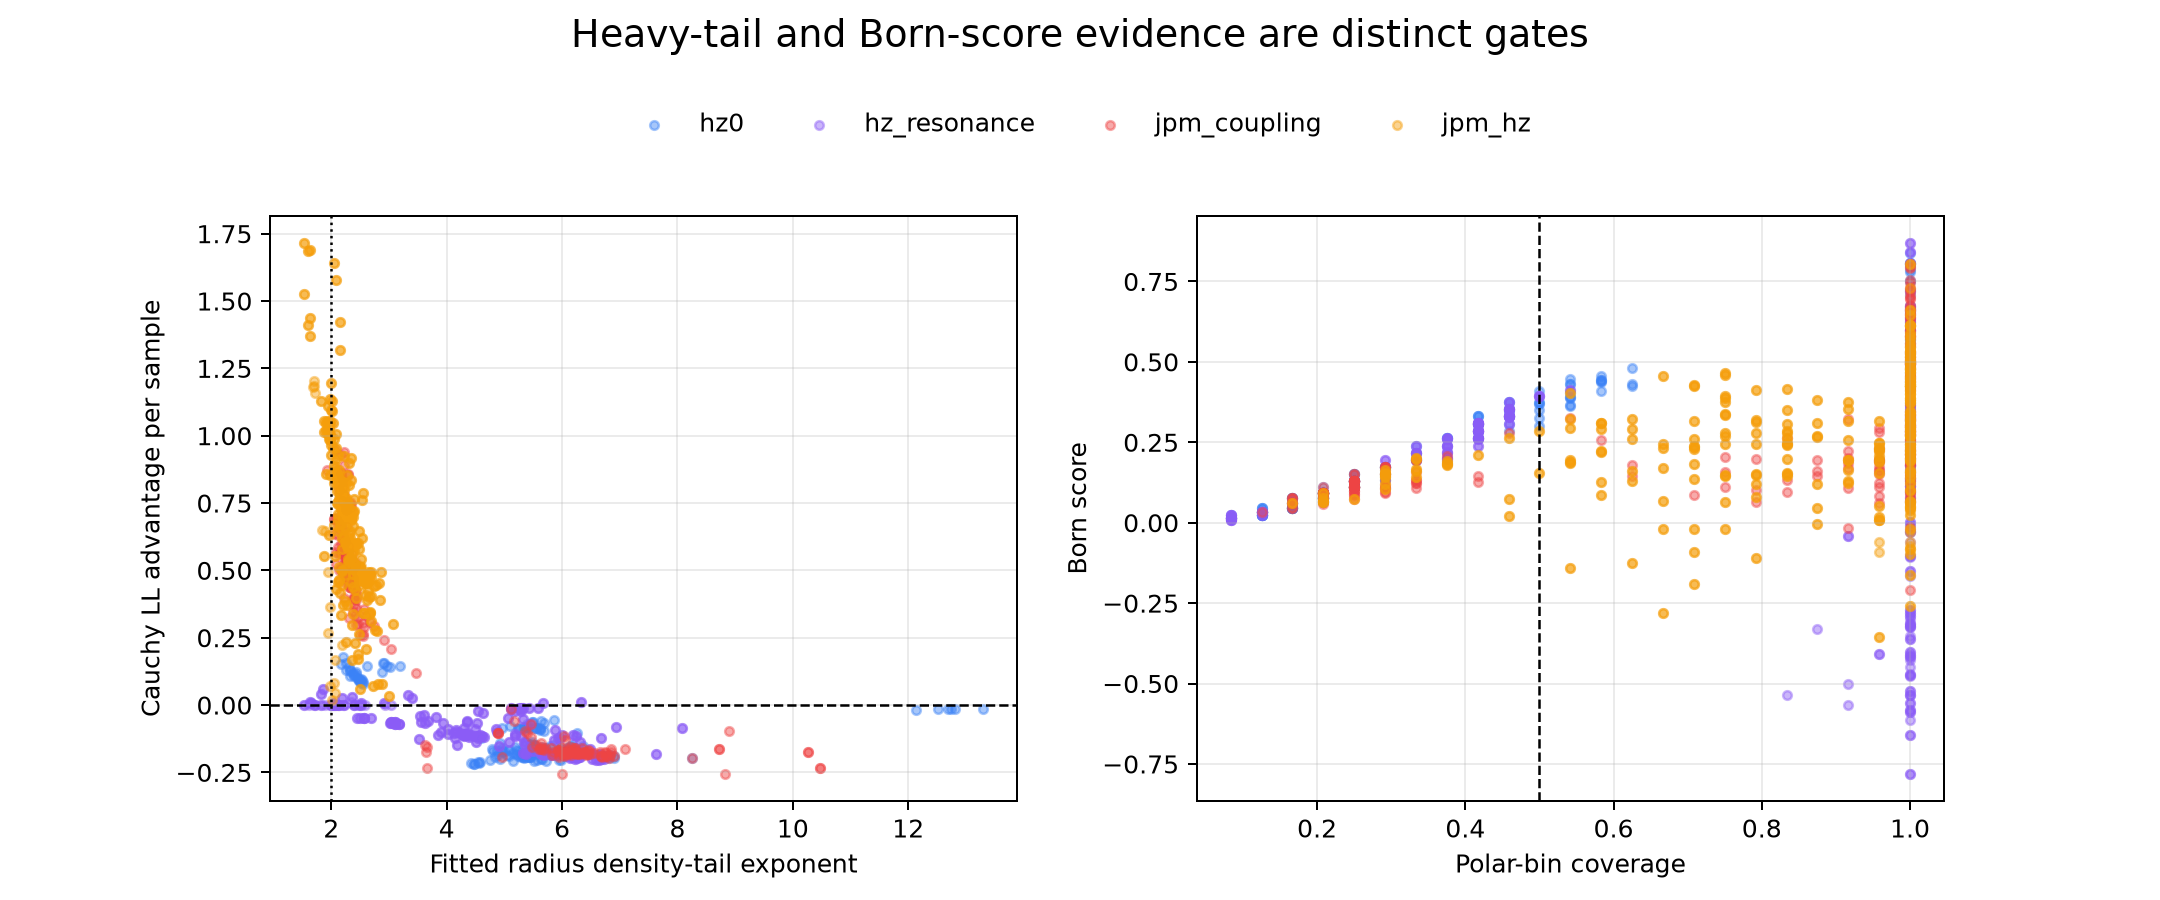
\includegraphics[width=0.86\textwidth]{regime_tradeoffs.png}
\caption{\textbf{Post-cutoff control atlas.}  Across 1,208 spectra, radial heavy-tail evidence, polar coverage, and the polar Born score are distinct diagnostics.  Resonance and exchange families can show high polar scores while remaining nearly meridional.  This descriptive figure is not a causal classifier and supplies no error bars.}
\label{sfig:controls}
\end{figure}

\section{Interpretive boundary and submission-critical checks}

Established exactly are the forward matrix-pencil reduction, antipodal outcome duality, regular projective root count, generic nonadditivity of the product intersection, the inverse-time production bridge, and the Haar spherical-ensemble law.  Established numerically within the stated finite datasets are the matched-ring size trend, the full-sphere binned diagnostics, and the control separation in Fig.~\ref{sfig:controls}.

Not established are an operational probability measure over roots and detector rays; a common apparatus-ready macrostate; stable, distinguishable, redundant detector records; homogeneous-QZ residual and conditioning validation of the production-scale roots; controlled $N\to\infty$, time-window, or resolution convergence; or a Hamiltonian-level mechanism explaining the matched condition.  In particular, algebraic multiplicity is only a provisional counting convention.  Spectral-statistics and chaos claims are excluded because the relevant spectra have not received the symmetry-sector and ensemble controls required for that inference~\cite{Atas2013}.

The actionable missing calculations are maintained in \texttt{RESULTS\_NEEDED.md}.  The two most consequential are:
\begin{enumerate}
\item \resultneeded{derive a normalized preparation/selection measure over qubit roots, detector null rays, degeneracies, and readout times without fitting the Born target};
\item \resultneeded{demonstrate that the associated detector factors form stable, distinguishable, preferably redundant record sectors over a nonzero time window}.
\end{enumerate}
Without these results, the paper establishes measurement-compatible unitary geometry and Born-like root counts, not a completed ontology of definite outcomes.

\bibliography{references}
\end{document}
